
\section{Benchmark IS}
Celem eksperymentów była ocena efektywności implementacji algorytmu sortowania całkowitoliczbowego (Integer Sort, IS) w czterech wersjach programistycznych (new\_omp, old\_omp, tbb, rust) przy różnych klasach problemów (S, W, A, B) i liczbie wątków. Porównanie obejmuje czas wykonania, wydajność (MFLOPS) oraz współczynnik zmienności (CV - coefficient of variation), obrazujący stabilność pomiarową.

\subsection{Wyniki benchmarków - platforma ARM64}
\begin{figure}[H]
    \centering
    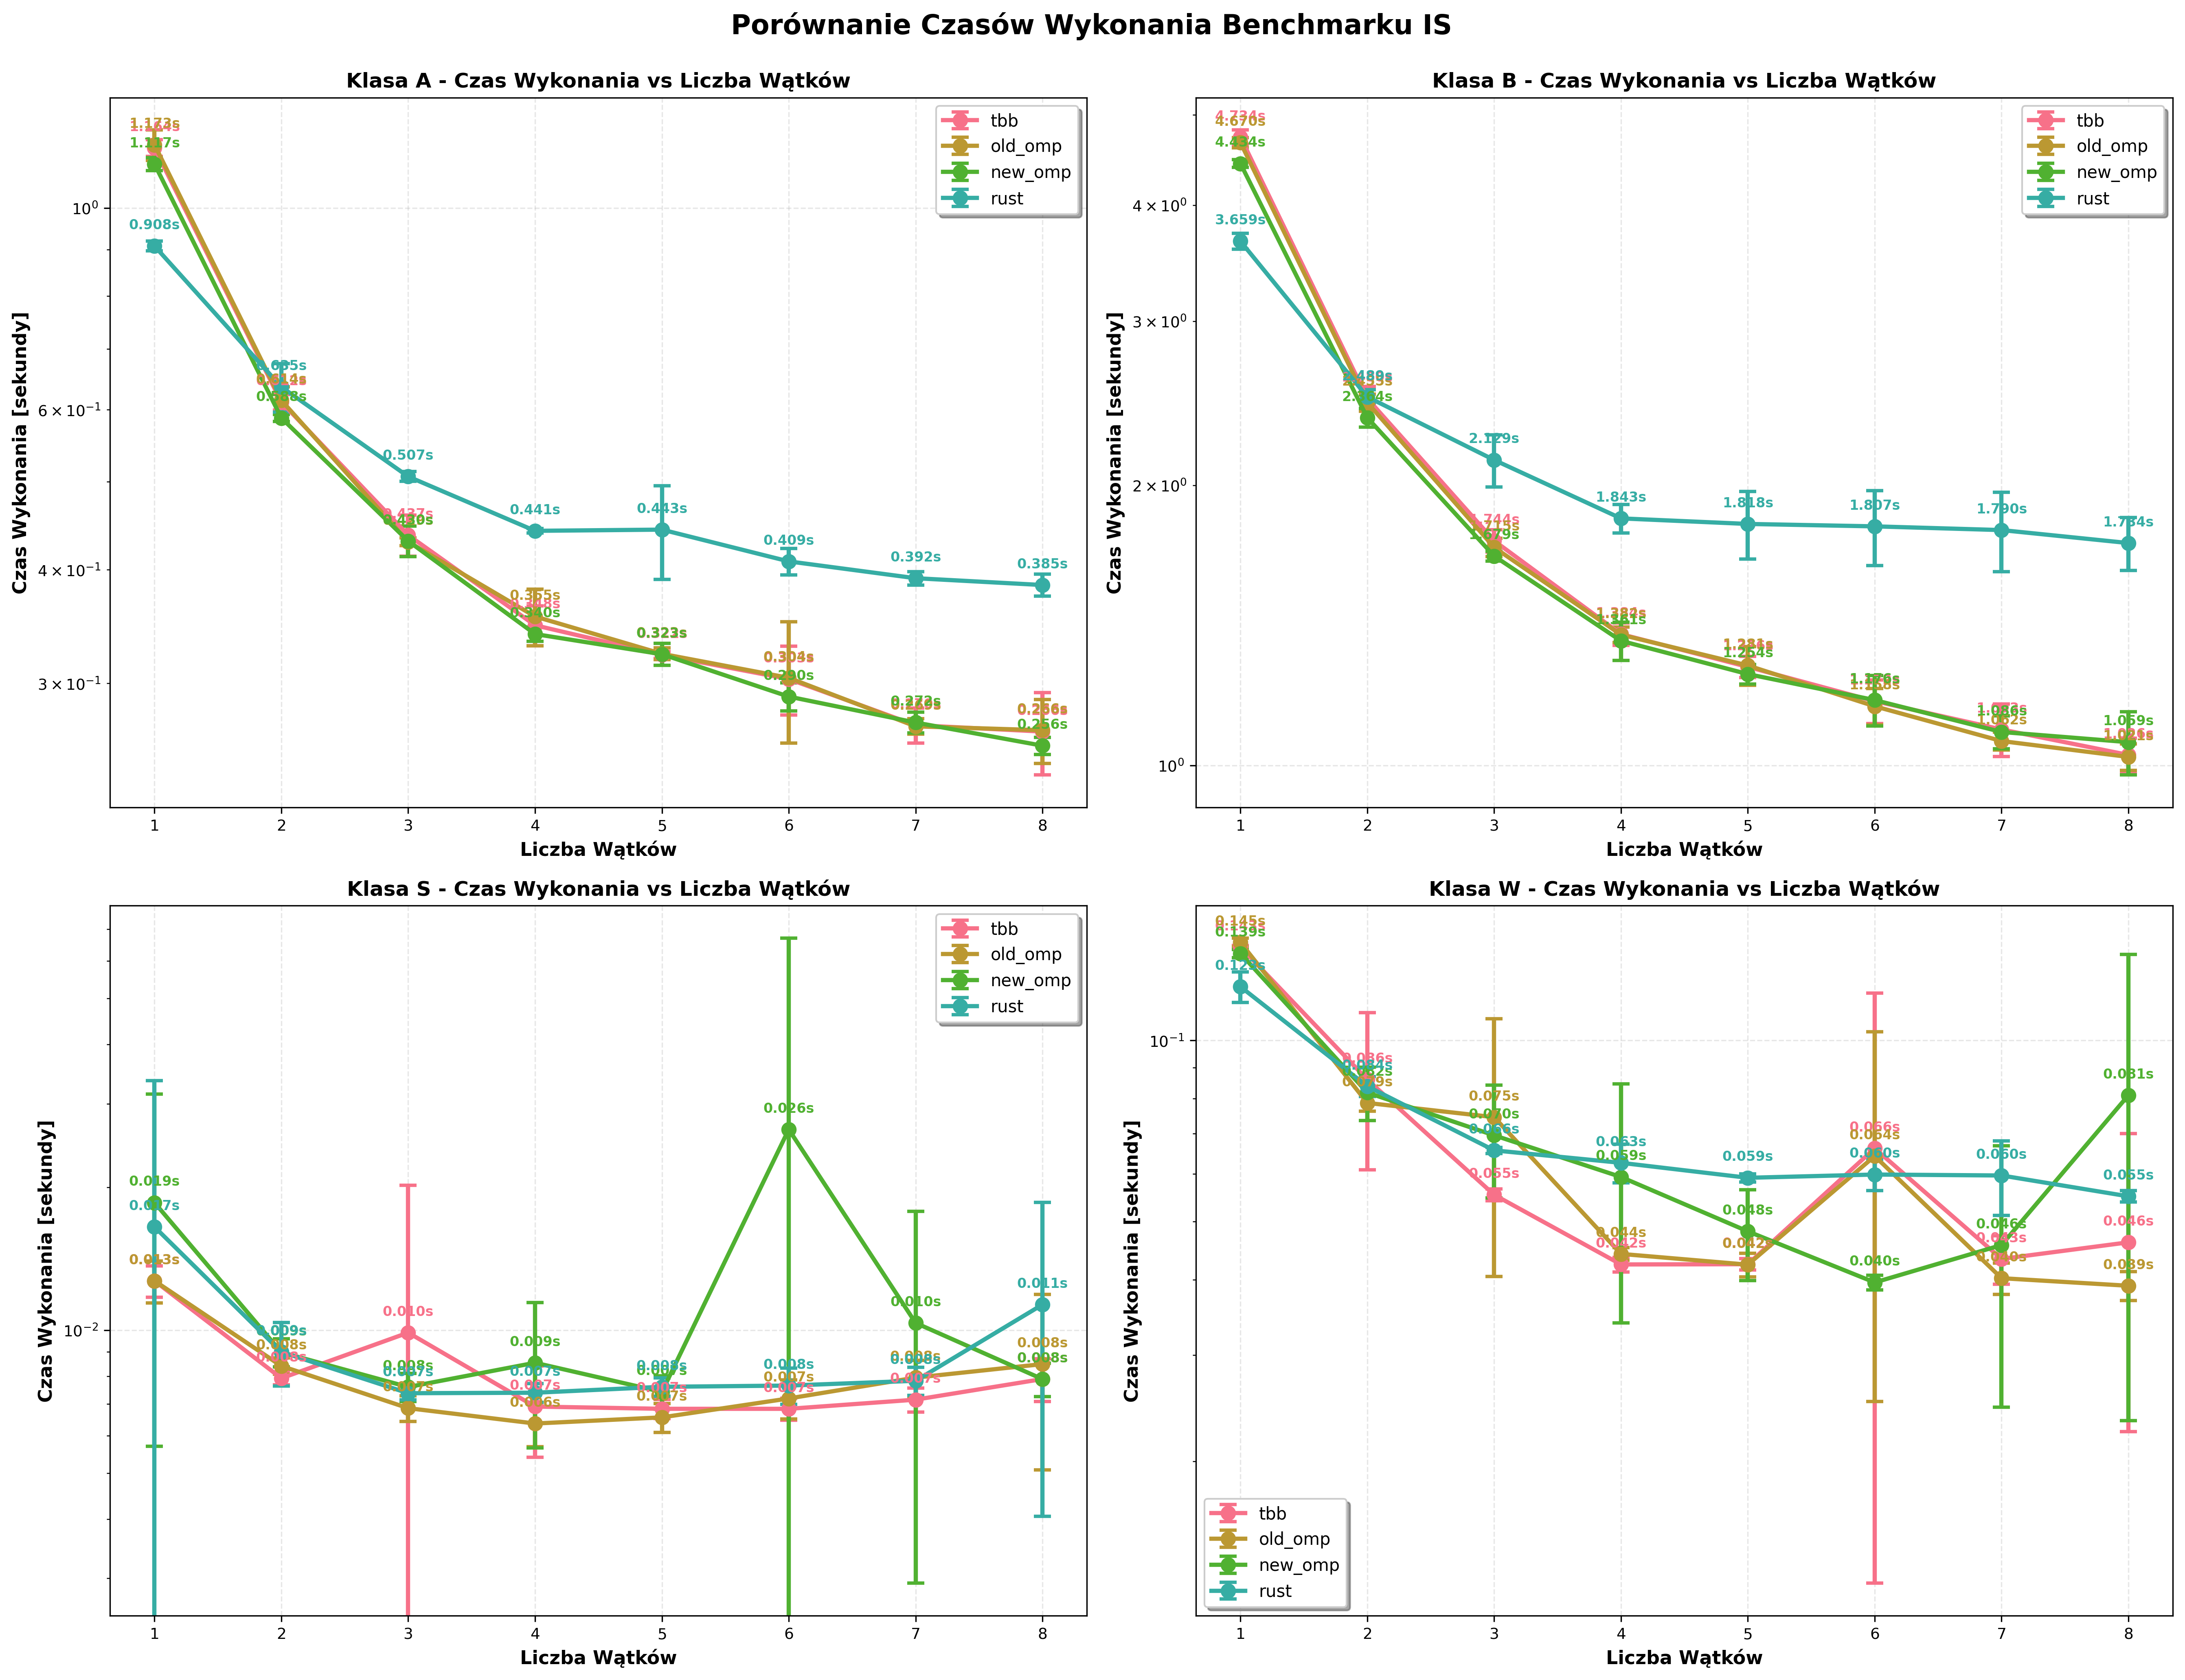
\includegraphics[width=\textwidth]{analiza/images/parallel/is/is_porownanie_czasow_wykonania.png}
    \caption{Porównanie czasów wykonania benchmarku IS dla klas S, W, A, B względem liczby użytych wątków}
    \label{is_porownanie_czasow_wykonania}
\end{figure}

Wszystkie cztery wykresy na rysunku przedstawiają zależność między czasem wykonania a liczbą wątków dla poszczególnych klas problemu.
\begin{itemize}
    \item W klasach A i B wszystkie implementacje wykazują bardzo dobrą skalowalność. W szczególności tbb, old\_omp oraz new\_omp charakteryzują się podobnymi i niskimi czasami wykonania (poniżej 0,2 sekundy), z zauważalną poprawą przy zwiększaniu liczby wątków.
    \item rust, mimo wyraźnie wyższego czasu wykonania we wszystkich klasach, wykazuje poprawę skalowalności, chociaż jej krzywe wykazują tendencję do wypłaszczania już od 4 wątków.
    \item Dla klas S i W, czasy wykonania są niewielkie, jednak większe odchylenia (widoczne na słupkach błędów) wskazują na trudności w utrzymaniu stabilnej równoległości przy mniejszych rozmiarach danych.
\end{itemize}



\begin{figure}[H]
    \centering
    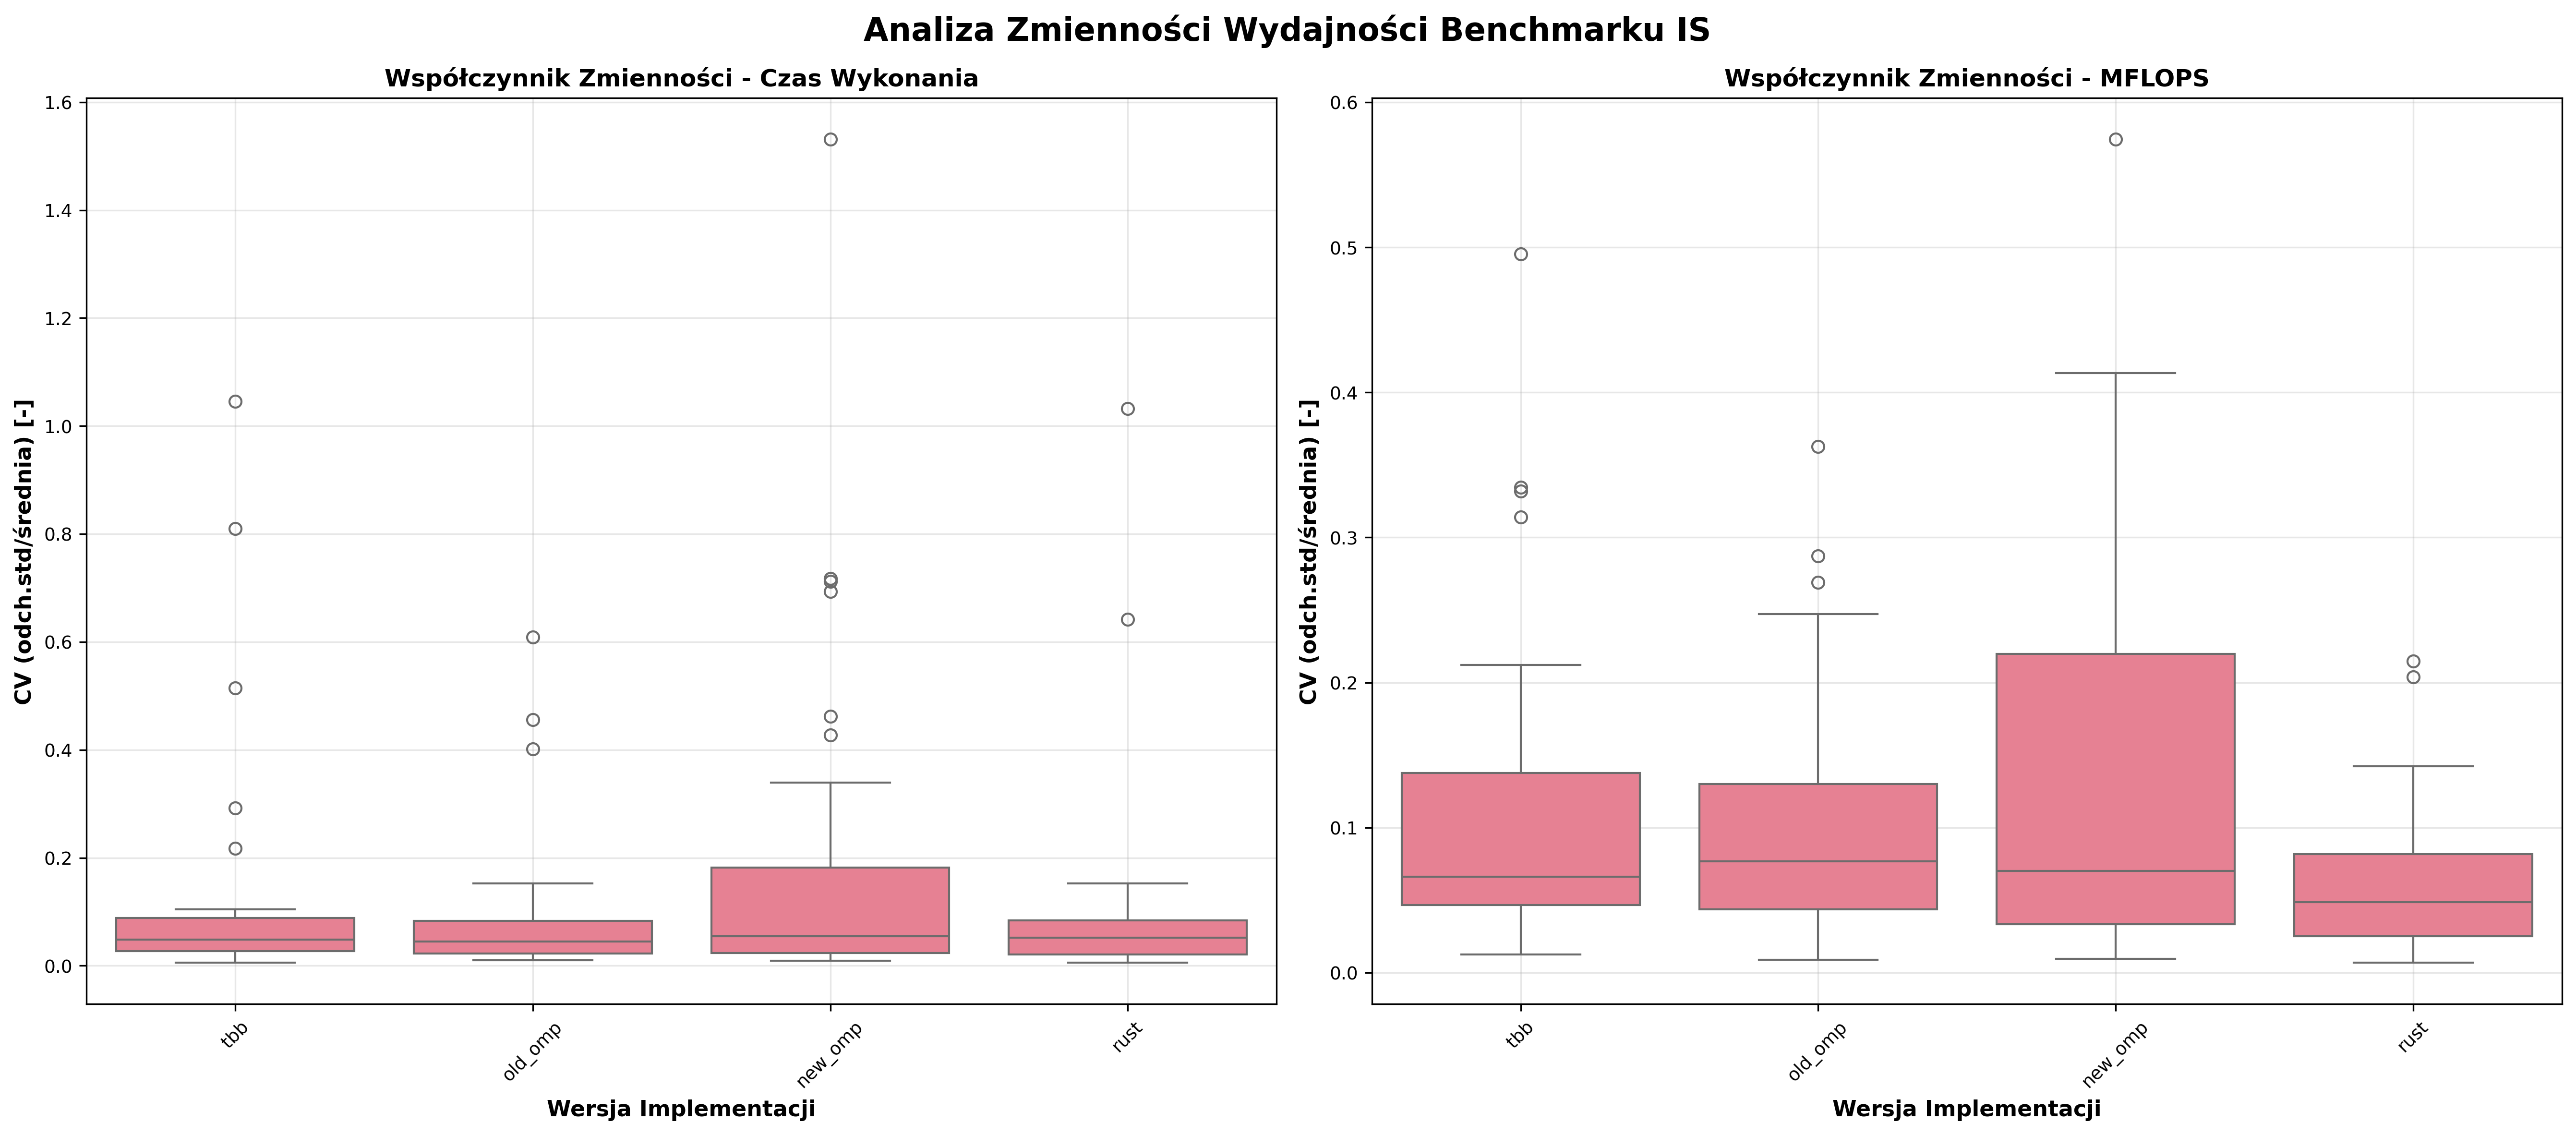
\includegraphics[width=\textwidth]{analiza/images/parallel/is/is_analiza_zmiennosci.png}
    \caption{Analiza zmienności czasów wykonania benchmarku IS dla klas S, W, A, B względem liczby użytych wątków}
    \label{is_analiza_zmiennosci}
\end{figure}
\begin{itemize}
    \item Najniższe wartości CV zarówno dla czasu wykonania, jak i MFLOPS zaobserwowano w implementacji rust, co wskazuje na najwyższą stabilność działania.
    \item tbb i old\_omp również wykazują dobrą stabilność, z medianą CV < 0,1.
    \item new\_omp, mimo wysokiej wydajności, charakteryzuje się większą zmiennością, zwłaszcza w MFLOPS, gdzie wartości CV osiągają nawet 0,5 w pojedynczych przypadkach. Może to świadczyć o niestabilnym zarządzaniu zasobami lub większym wpływie środowiska wykonawczego.
\end{itemize}



%------------------------------
\begin{figure}[H]
    \centering
    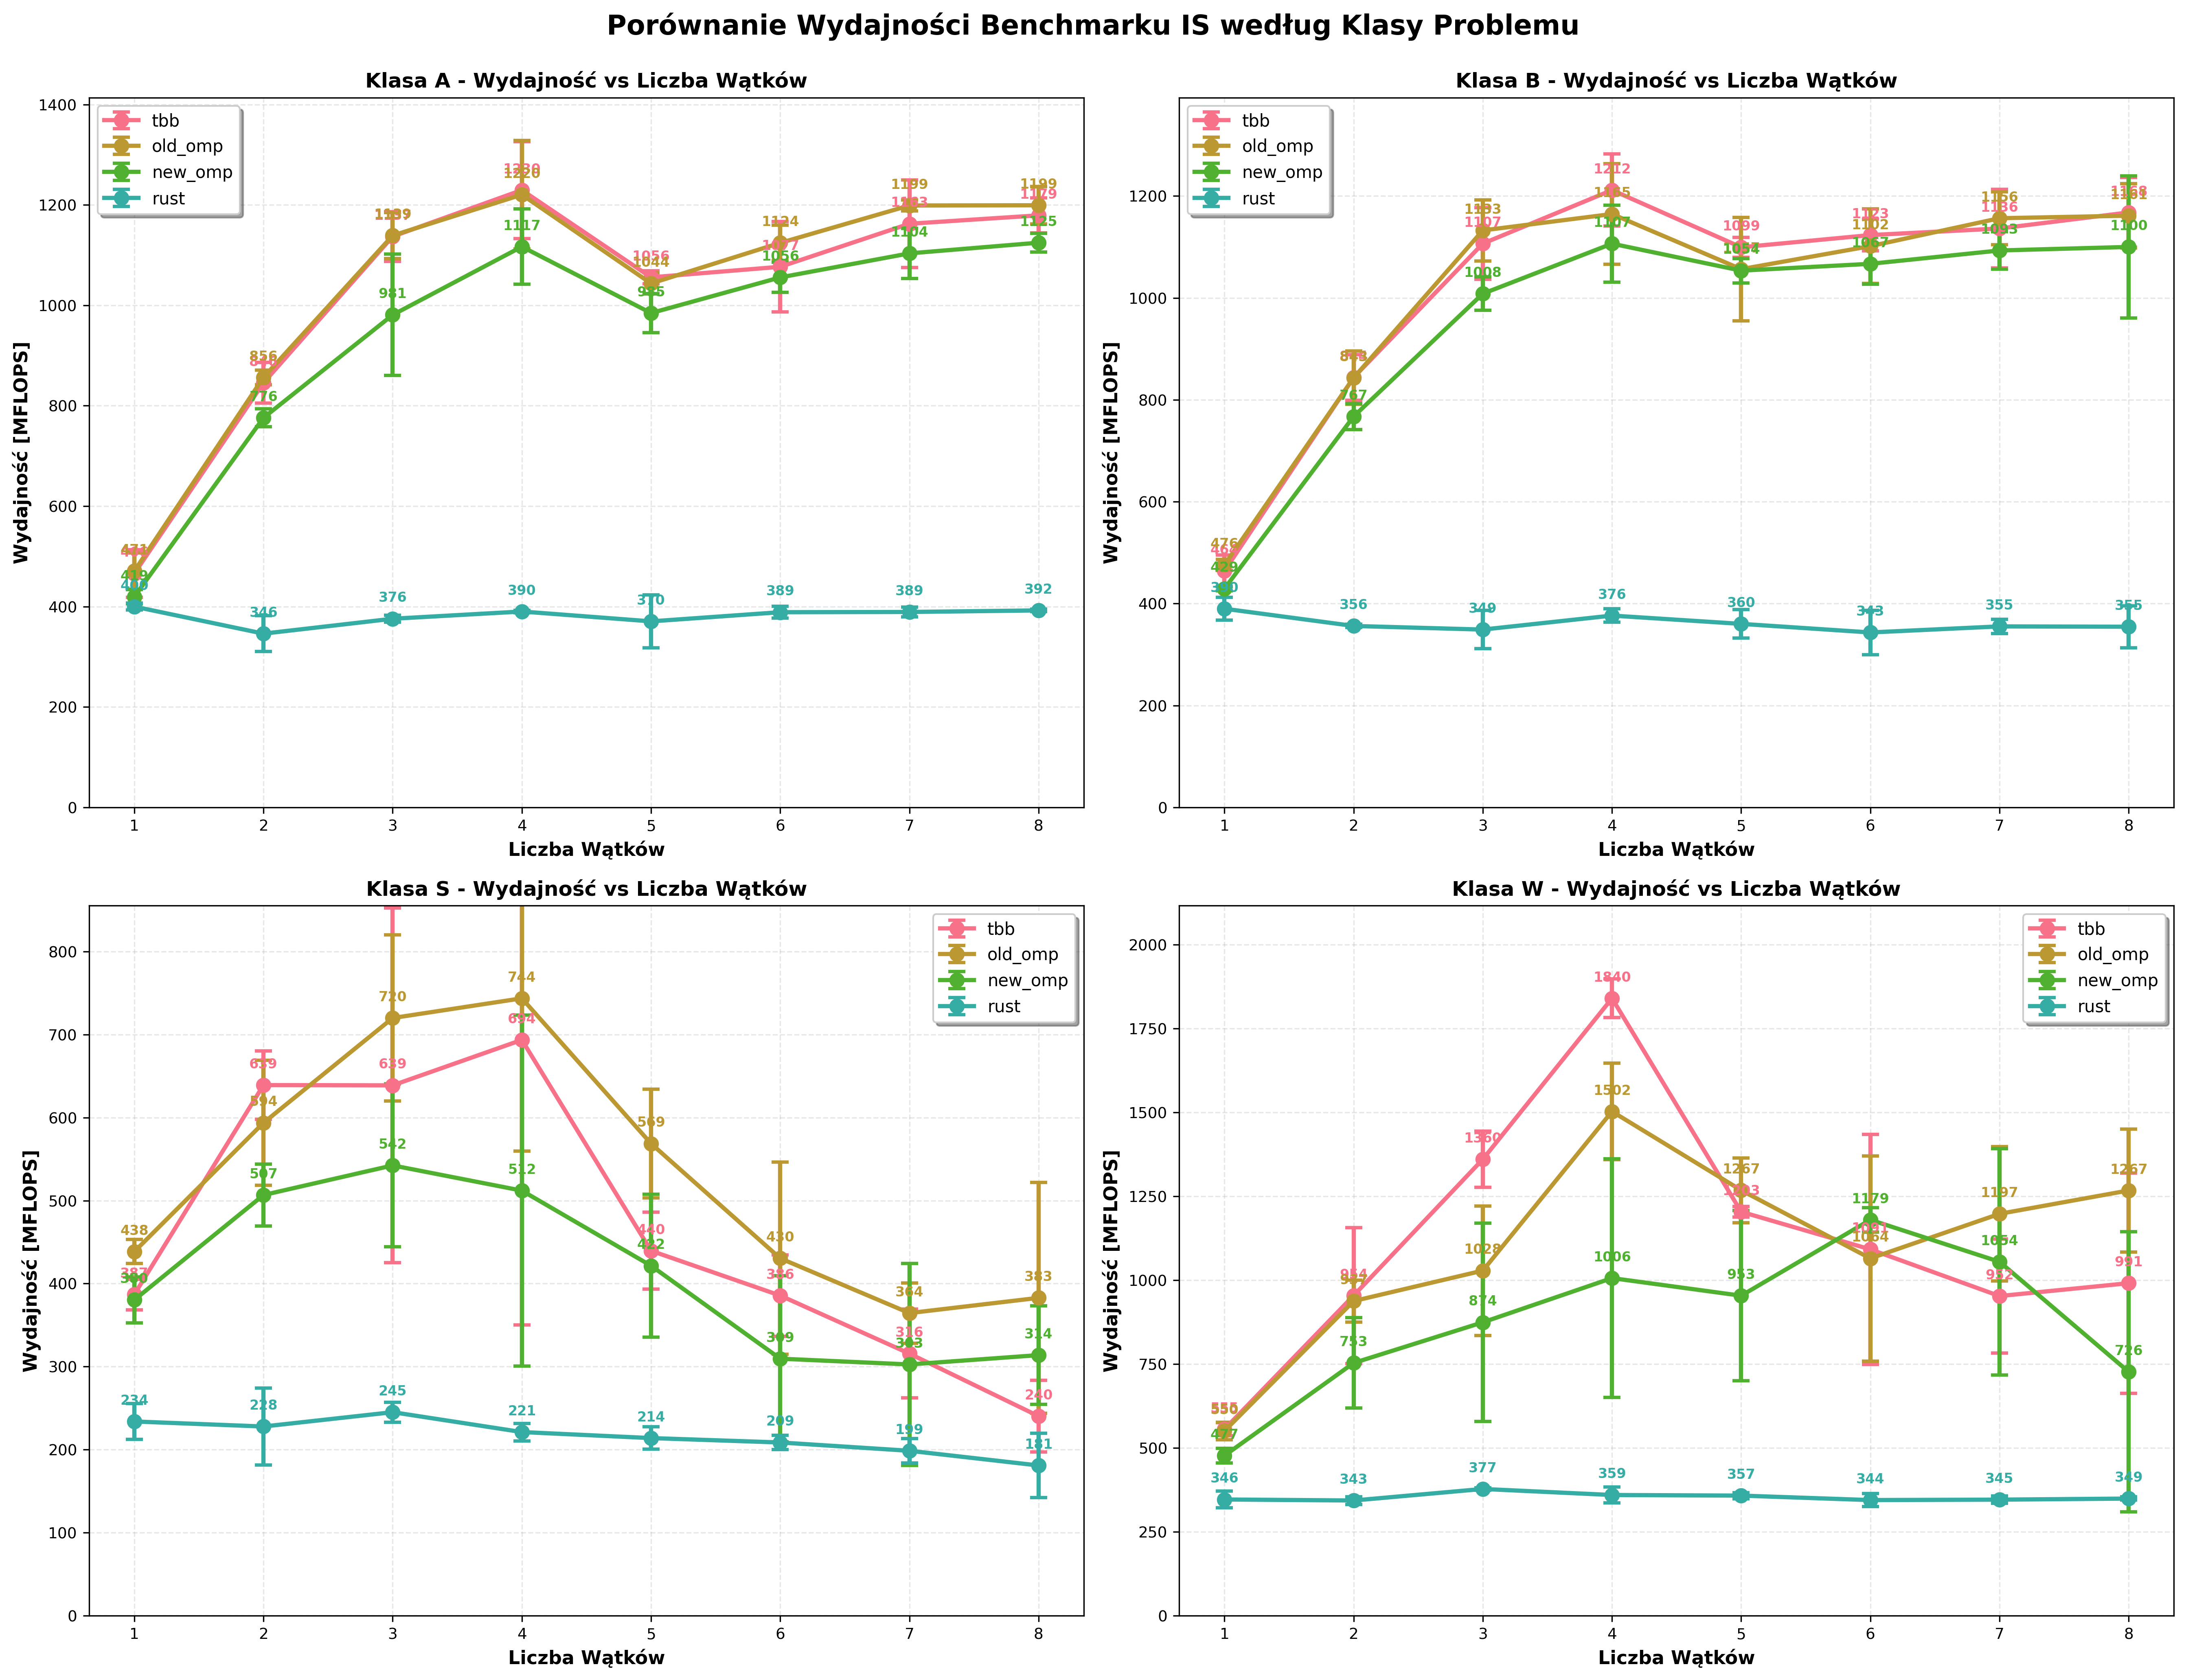
\includegraphics[width=\textwidth]{analiza/images/parallel/is/is_porownanie_wydajnosci.png}
    \caption{Porównanie wydajności benchmarku IS dla klas S, W, A, B względem liczby użytych wątków}
    \label{is_porownanie_wydajnosci}
\end{figure}
Na wykresach na rysunku \ref{ep_porownanie_wydajnosci} zaprezentowano porównanie wydajności benchmarku IS mierzonej w MFLOPS (milionach operacji zmiennoprzecinkowych na sekundę). Wydajność została przedstawiona jako funkcja liczby wątków (1-8) dla czterech implementacji równoległych.
\begin{itemize}
    \item Dla klas A i B, tbb oraz old\_omp osiągają wartości przekraczające 1300 MFLOPS przy 4 wątkach, co stanowi bardzo dobrą charakterystykę. new\_omp utrzymuje się tuż za nimi.
    \item rust, mimo że znacznie wolniejszy czasowo, prezentuje stabilną, lecz niską wydajność rzędu 350-390 MFLOPS niezależnie od liczby wątków. Może to sugerować, że implementacja nie skaluje się efektywnie lub operuje z istotnym narzutem.
    \item W klasach S i W zauważalne są spadki wydajności po osiągnięciu 4 wątków. Dla tbb oraz old\_omp pojawia się zjawisko tzw. nadmierna równoległość \eng{over-parallelization}, gdzie narzut synchronizacji przewyższa zysk z dodatkowej równoległości.
\end{itemize}



\begin{figure}[H]
    \centering
    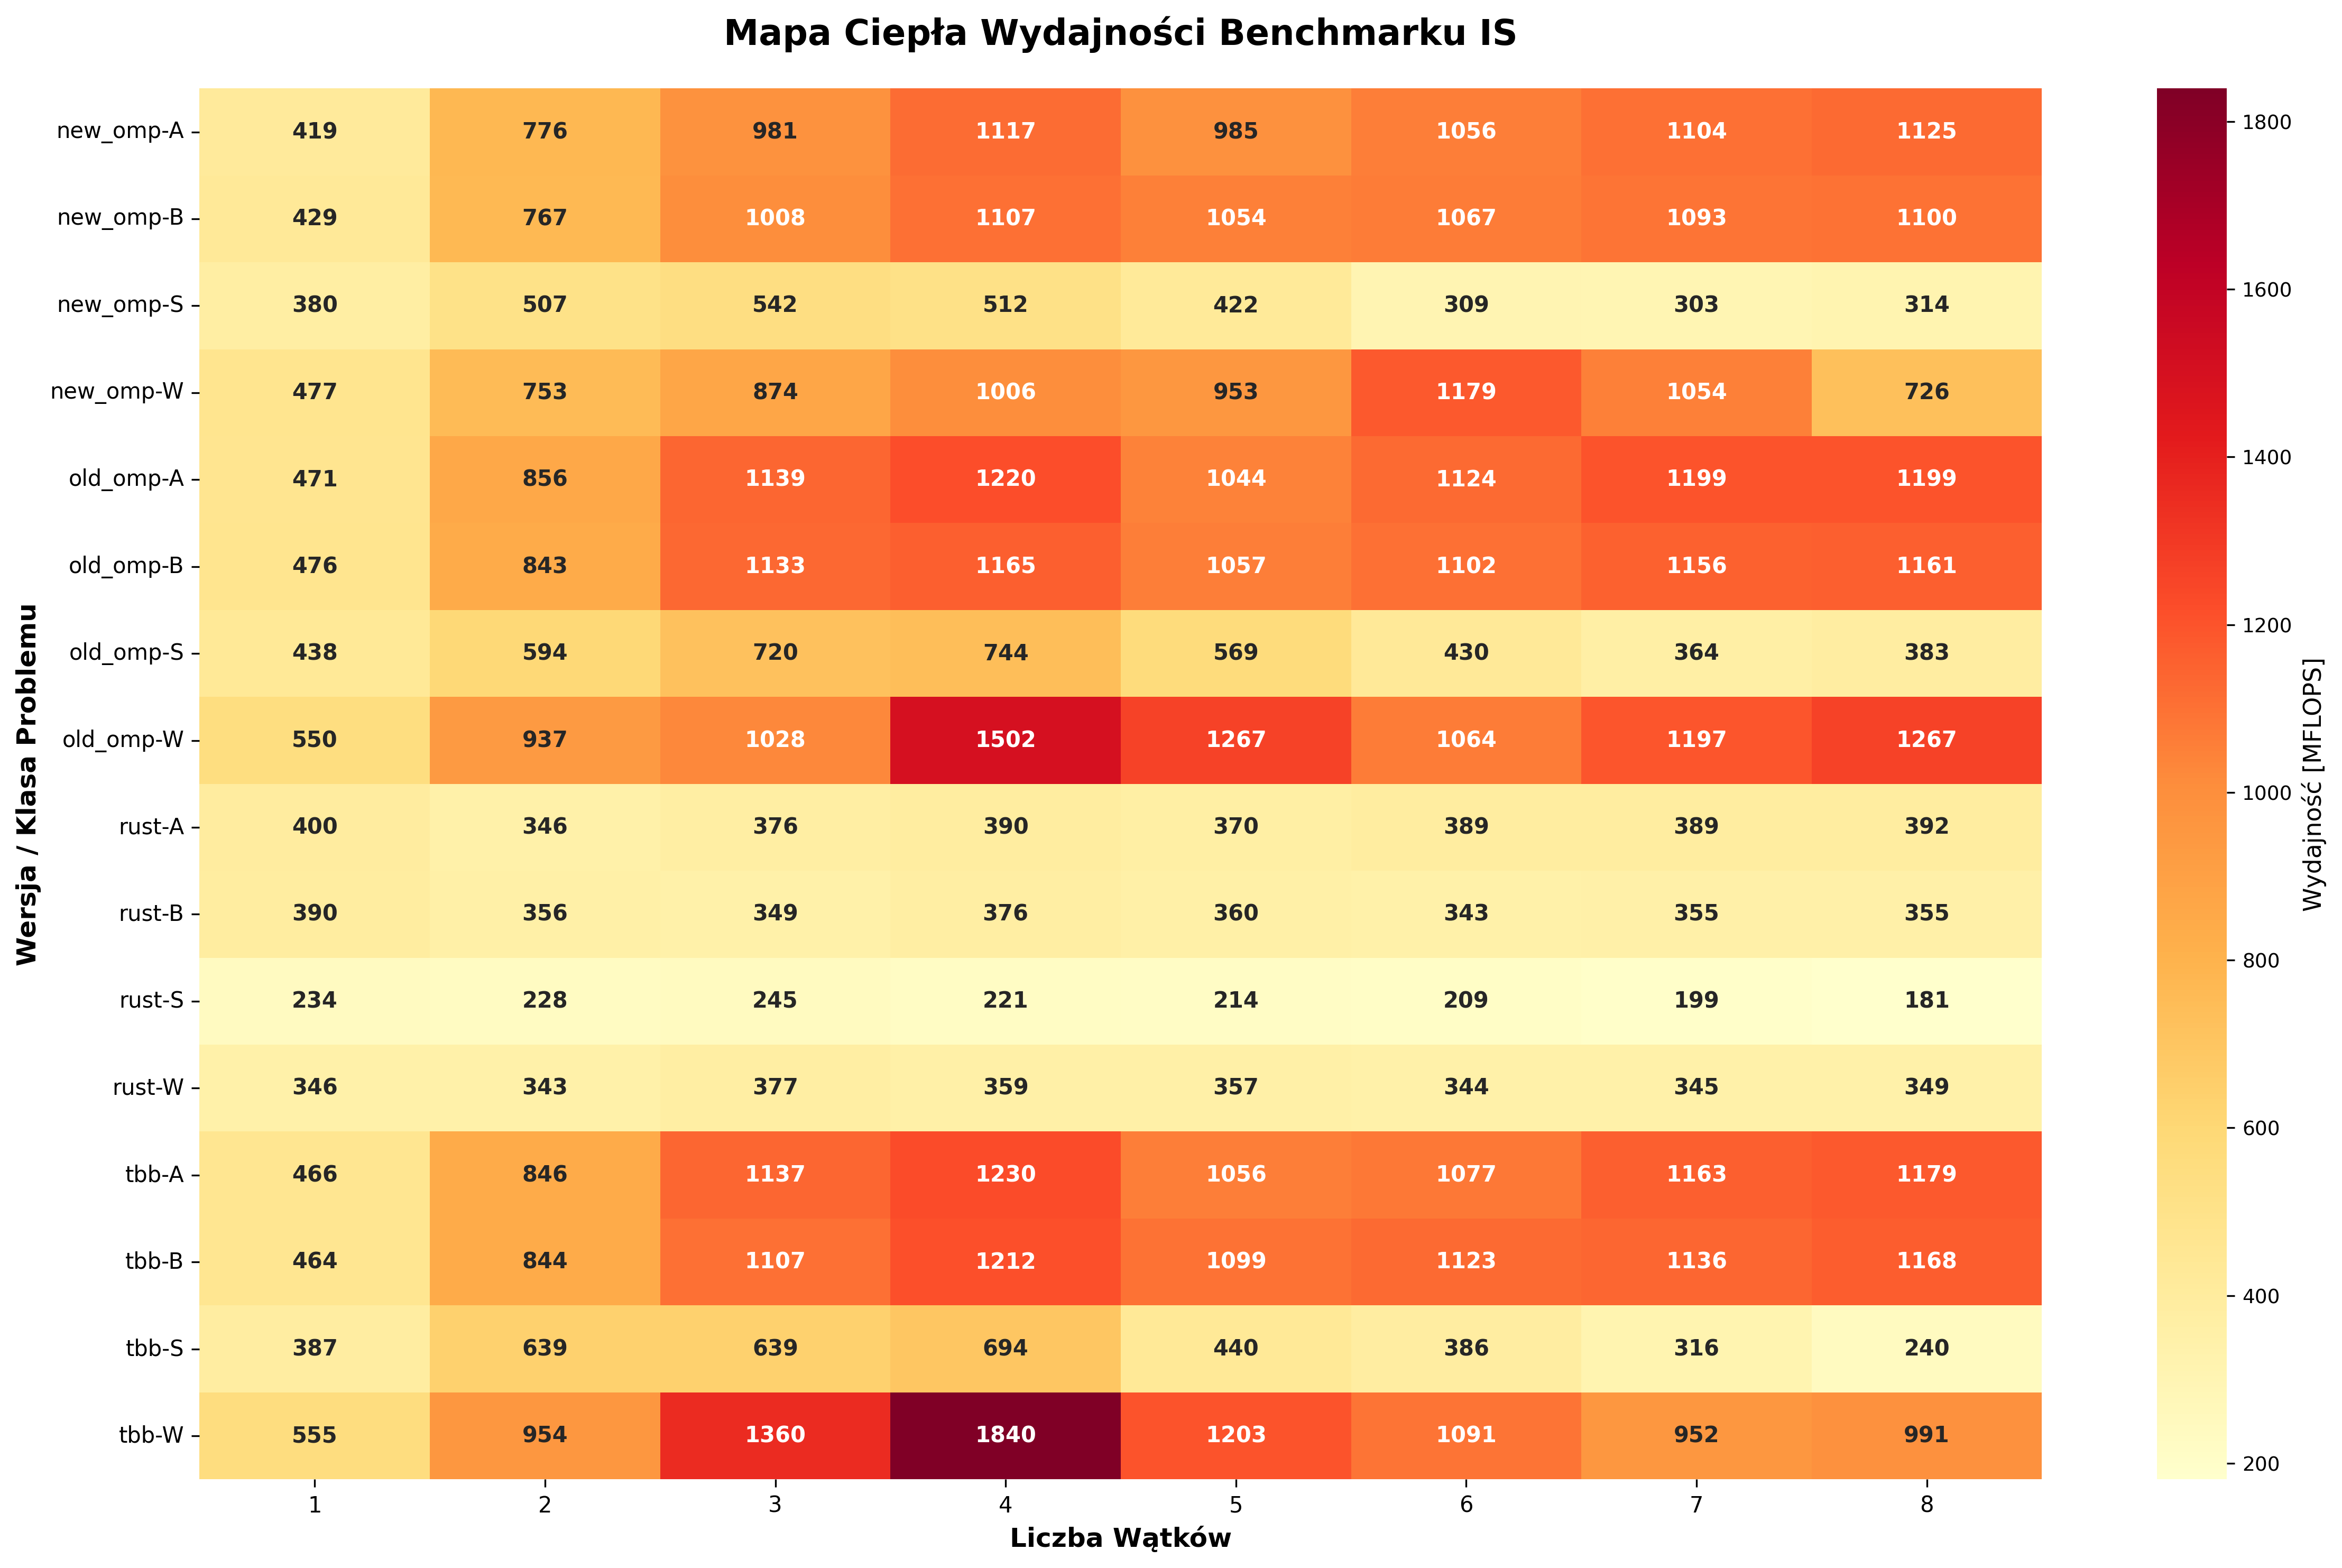
\includegraphics[width=\textwidth]{analiza/images/parallel/is/is_mapa_ciepla_wydajnosci.png}
    \caption{Mapa ciepła wydajności benchmarku IS dla klas S, W, A, B względem liczby użytych wątków}
    \label{is_heatmap_wydajnosci}
\end{figure}
Powyższa mapa cieplna - rysunek \ref{ep_heatmap_wydajnosci} przedstawia wydajność (w MFLOPS). Wydajność została przedstawiona w zależności od liczby użytych wątków. Odcienie koloru od żółtego do ciemnoczerwonego wskazują na wzrost wydajności.
\begin{itemize}
    \item Najwyższe wartości MFLOPS osiągnięto dla wersji tbb-W (klasa W, 4 wątki), osiągając maksymalnie 1840 MFLOPS. Jest to również najwyższy wynik spośród wszystkich testów.
    \item old\_omp oraz tbb konsekwentnie uzyskują wysoką wydajność w klasach A i B, szczególnie przy 4-6 wątkach, gdzie dominują wartości przekraczające 1100 MFLOPS.
    \item Wersje dla klasy S i W wykazują większe zróżnicowanie - m.in. tbb-W oraz old\_omp-W prezentują wysoką skalowalność, podczas gdy new\_omp-S i rust-S cechują się ograniczonym wzrostem lub wręcz spadkiem wydajności przy rosnącej liczbie wątków.
\end{itemize}

\begin{figure}[H]
    \centering
    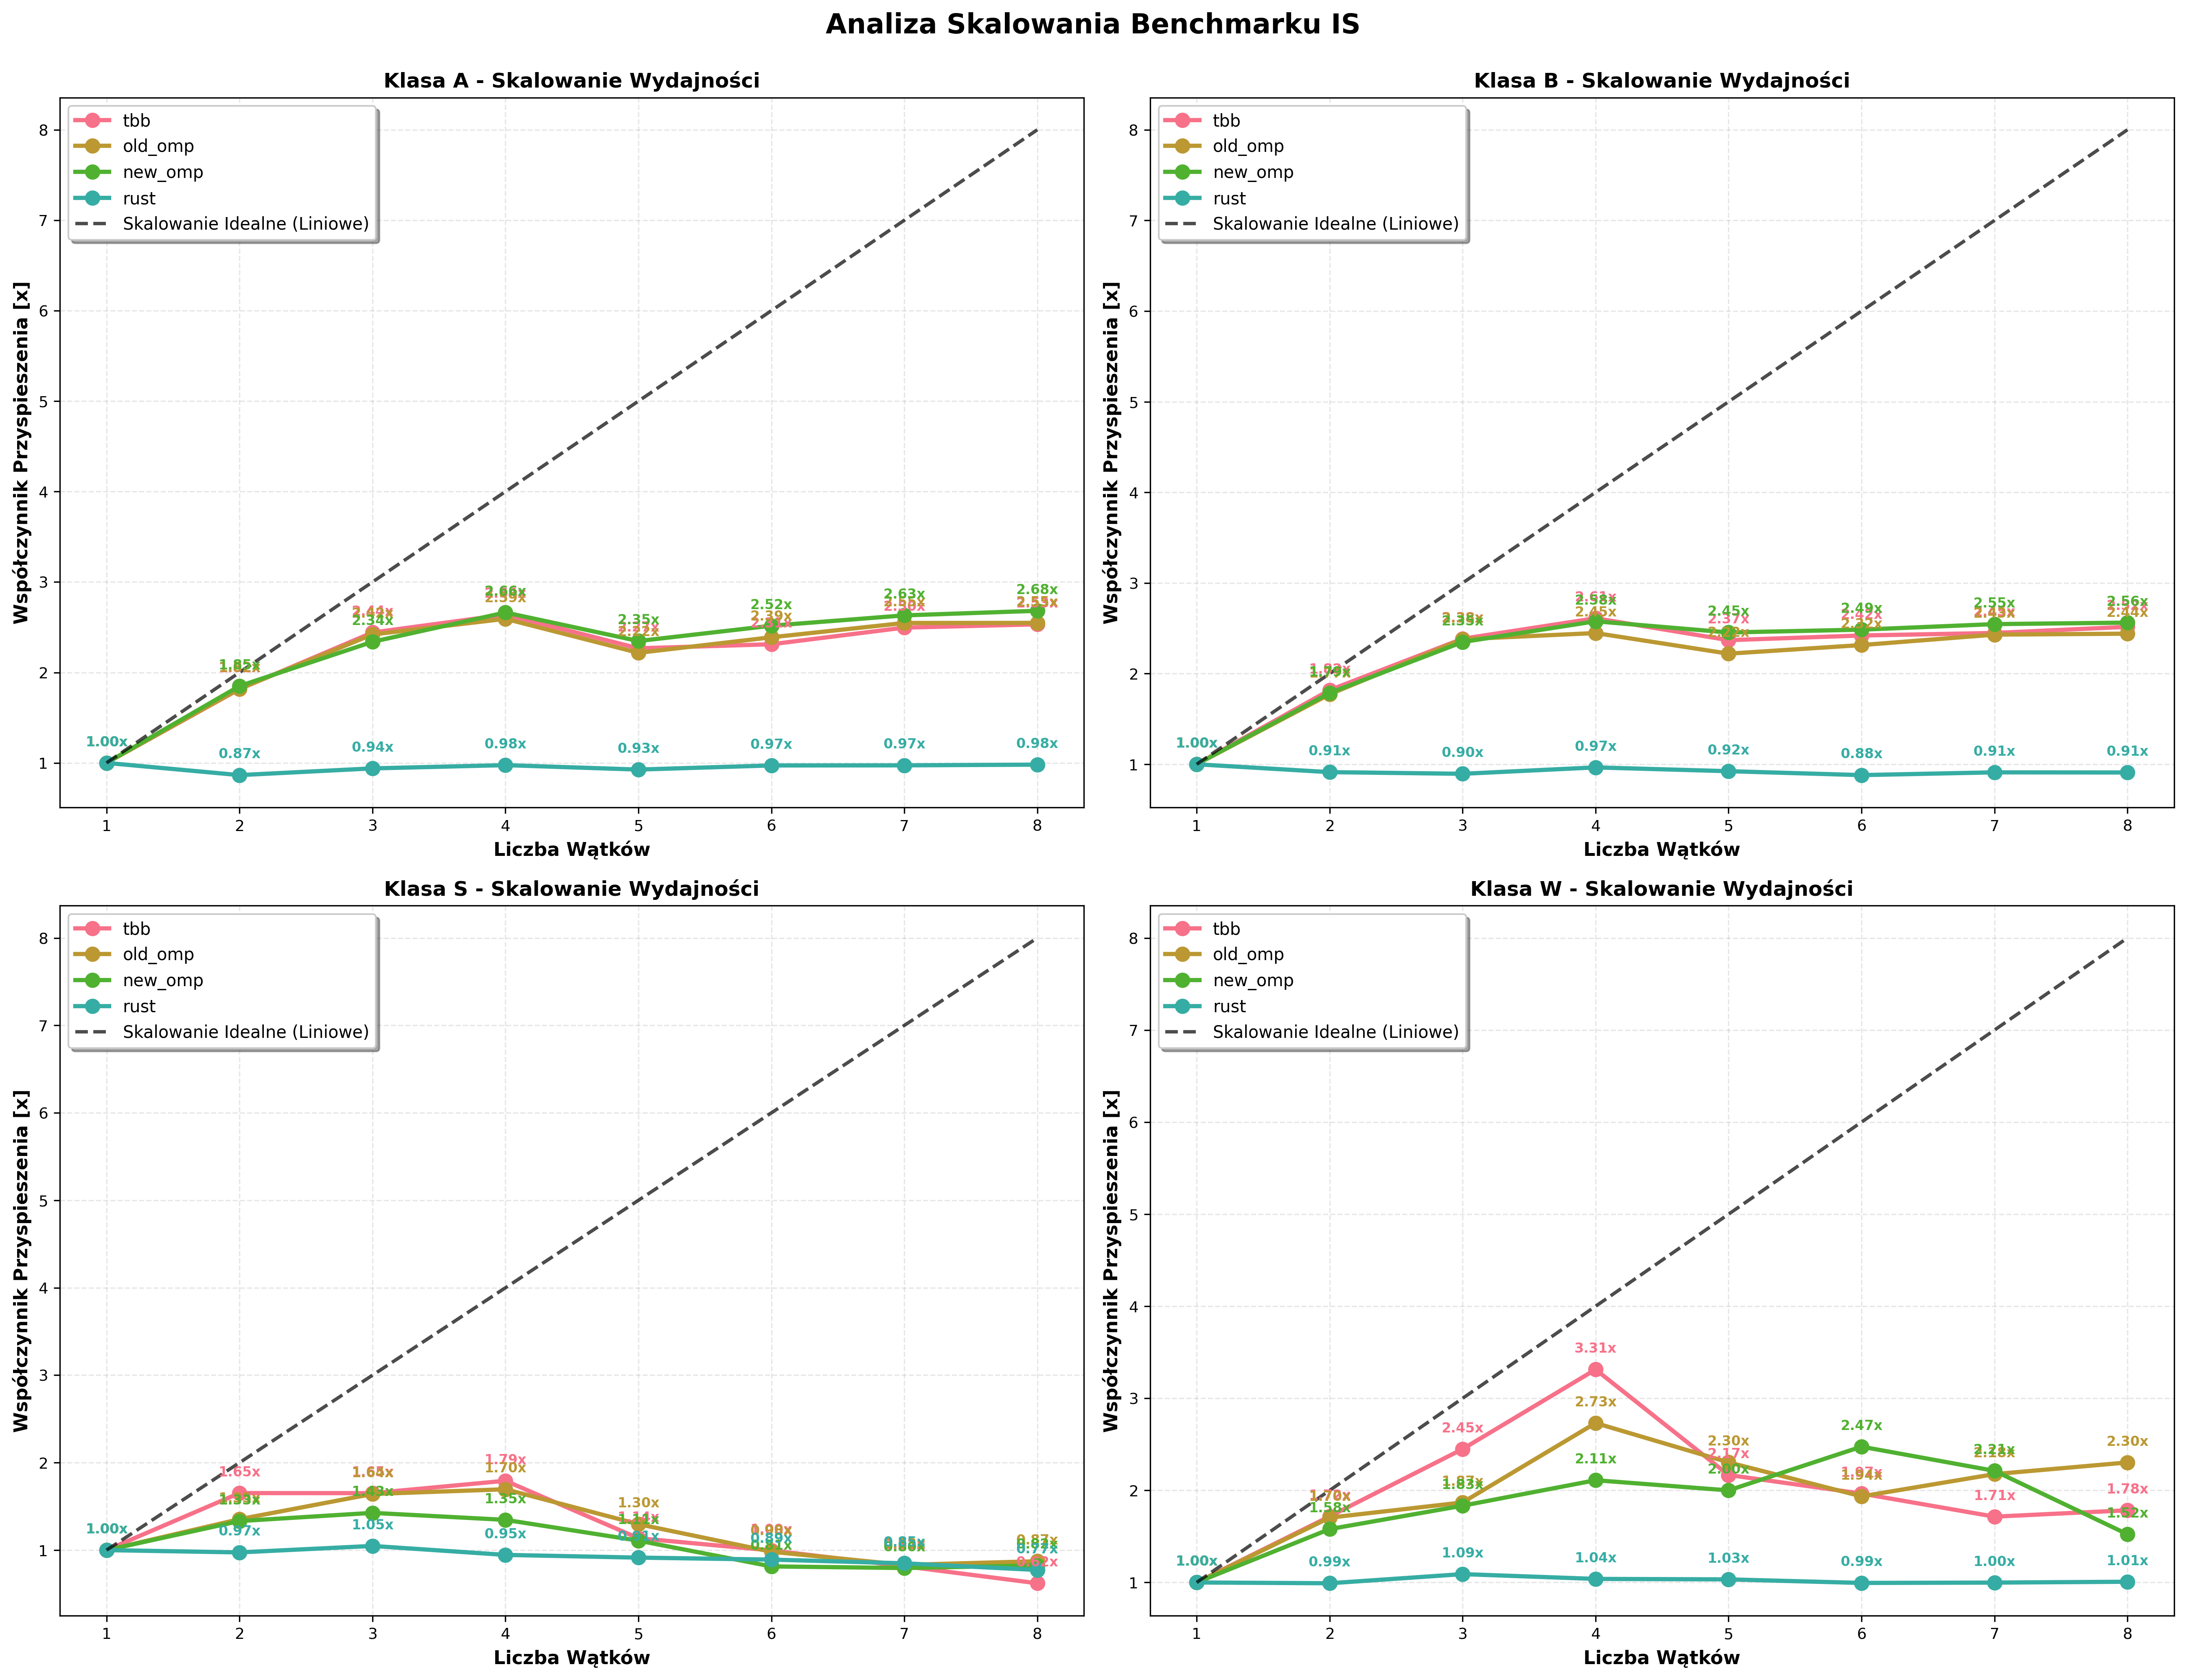
\includegraphics[width=\textwidth]{analiza/images/parallel/is/is_analiza_skalowania.png}
    \caption{Analiza skalowania benchmarku IS dla klas S, W, A, B względem liczby użytych wątków}
    \label{ip_analiza_skalowania}
\end{figure}
\subsubsection{Klasy A i B - skalowalność umiarkowana}
\begin{itemize}
    \item W klasach A i B, implementacje tbb, old\_omp i new\_omp uzyskują skalowalność w zakresie 2,5-2,6x przy 8 wątkach, co jest wynikiem umiarkowanym, lecz spójnym.
    \item Żadna z wersji nie osiąga skalowania liniowego. Jest to efektem m.in. ograniczeń algorytmu IS (o wysokiej zależności pamięciowej) oraz narzutów związanych z synchronizacją.
    \item Implementacja rust wykazuje znacznie słabsze skalowanie, które osiąga wartości tylko nieznacznie powyżej 1x, a nawet pogarsza się (np. 0,87x w klasie A przy 2 wątkach), co oznacza, że dodatkowe wątki nie tylko nie przyspieszają obliczeń, ale mogą je wręcz spowalniać
\end{itemize}


\subsection{Wyniki benchmarków - platforma x86\_64}
%------------------------------
%------------------------------
Aby lepiej zrozumieć charakterystyki pamięciowe testowanych implementacji benchmarku IS, przeprowadzono analizę zużycia pamięci, błędów stron pamięci oraz mechanizmu ich odzyskiwania. Wnioski wyciągnięto na podstawie trzech grup wykresów: bezwzględnych wartości (rys. \ref{is_porownanie_zuzycia_pamieci}), porównania względnego względem old\_omp (rys. \ref{is_analiza_wzgledem_old_omp}) oraz kompromisów między metrykami (rys. \ref{is_kompromisy_pamiec_bledy}).
\subsection{Wyniki profilowania wydajności - platforma ARM64}
\begin{figure}[H]
    \centering
    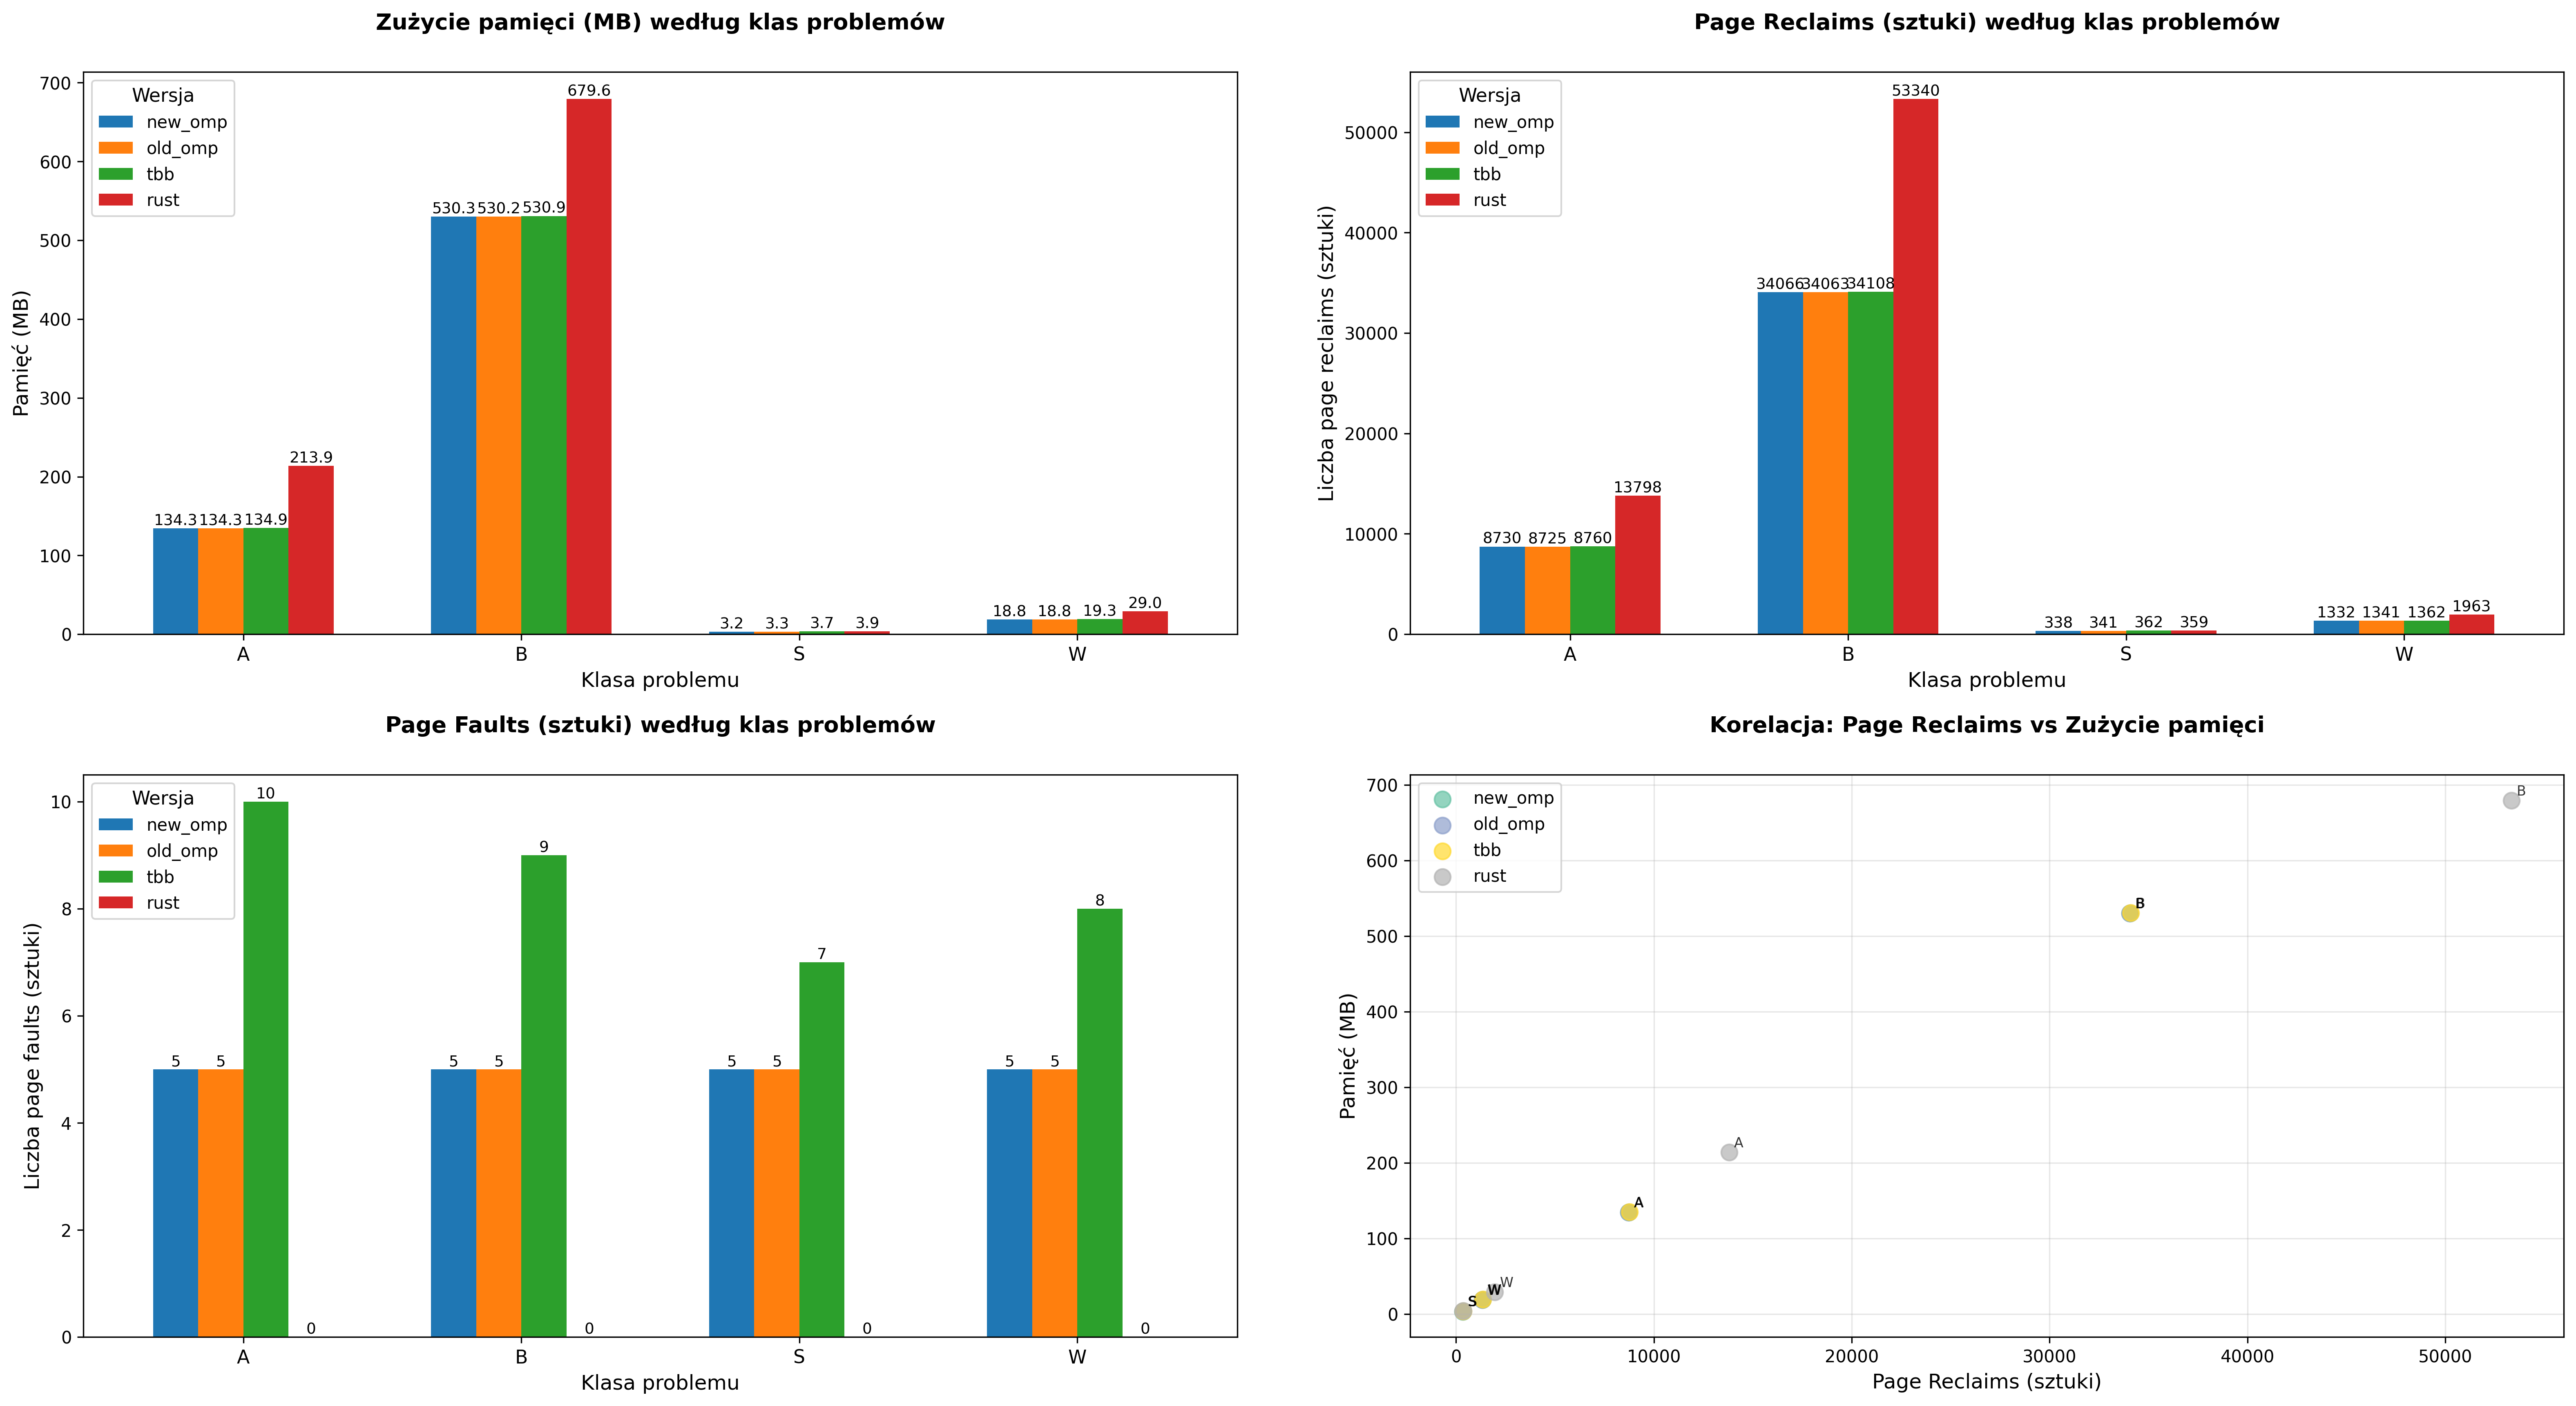
\includegraphics[width=\textwidth]{analiza/images/parallel/is/chart_01_memory_comparison.png}
    \caption{Profilowanie wydajności benchmarku IS dla klas S, W, A, B względem liczby użytych wątków}
    \label{is_porownanie_zuzycia_pamieci}
\end{figure}
\subsubsection{Zużycie pamięci i błędy stron}
Wykresy w górnym rzędzie przedstawiają bezwzględne zużycie pamięci oraz liczbę odzyskanych stron pamięci:
\begin{itemize}
    \item Największe zużycie pamięci odnotowano dla implementacji rust, osiągając 213,9 MB (klasa A) oraz 679,6 MB (klasa B). W pozostałych implementacjach (new\_omp, old\_omp, tbb) wartości te były niemal identyczne (np. ~134 MB w klasie A i ~530 MB w klasie B).
    \item Analogicznie, rust odzyskuje najwięcej stron, osiągając ponad 53 tysiące operacji w klasie B, co jest o ponad 50\% więcej niż w pozostałych wersjach. Sugeruje to intensywniejsze wykorzystanie dynamicznego zarządzania pamięcią lub częstsze zwalnianie obszarów.
    \item W zakresie błędów stron, rust jako jedyna implementacja nie generuje żadnych błędów stron (0 sztuk we wszystkich klasach), co potwierdza jej deterministyczne podejście do alokacji pamięci.
    \item Wersje new\_omp i old\_omp utrzymują stabilny poziom błędów (5 sztuk we wszystkich klasach), natomiast tbb wykazuje wyraźnie wyższy poziom błędów - od 7 do 10 sztuk.
\end{itemize}
W prawym dolnym wykresie zaprezentowano korelację między zużyciem pamięci a liczbą page reclaims. Wykres ujawnia wyraźną korelację dodatnią - implementacje i klasy, które zużywają więcej pamięci, zwalniają również więcej stron z pamięcią, co wynika z konieczności intensywniejszej obsługi zarządzania pamięcią operacyjną.

\begin{figure}[H]
    \centering
    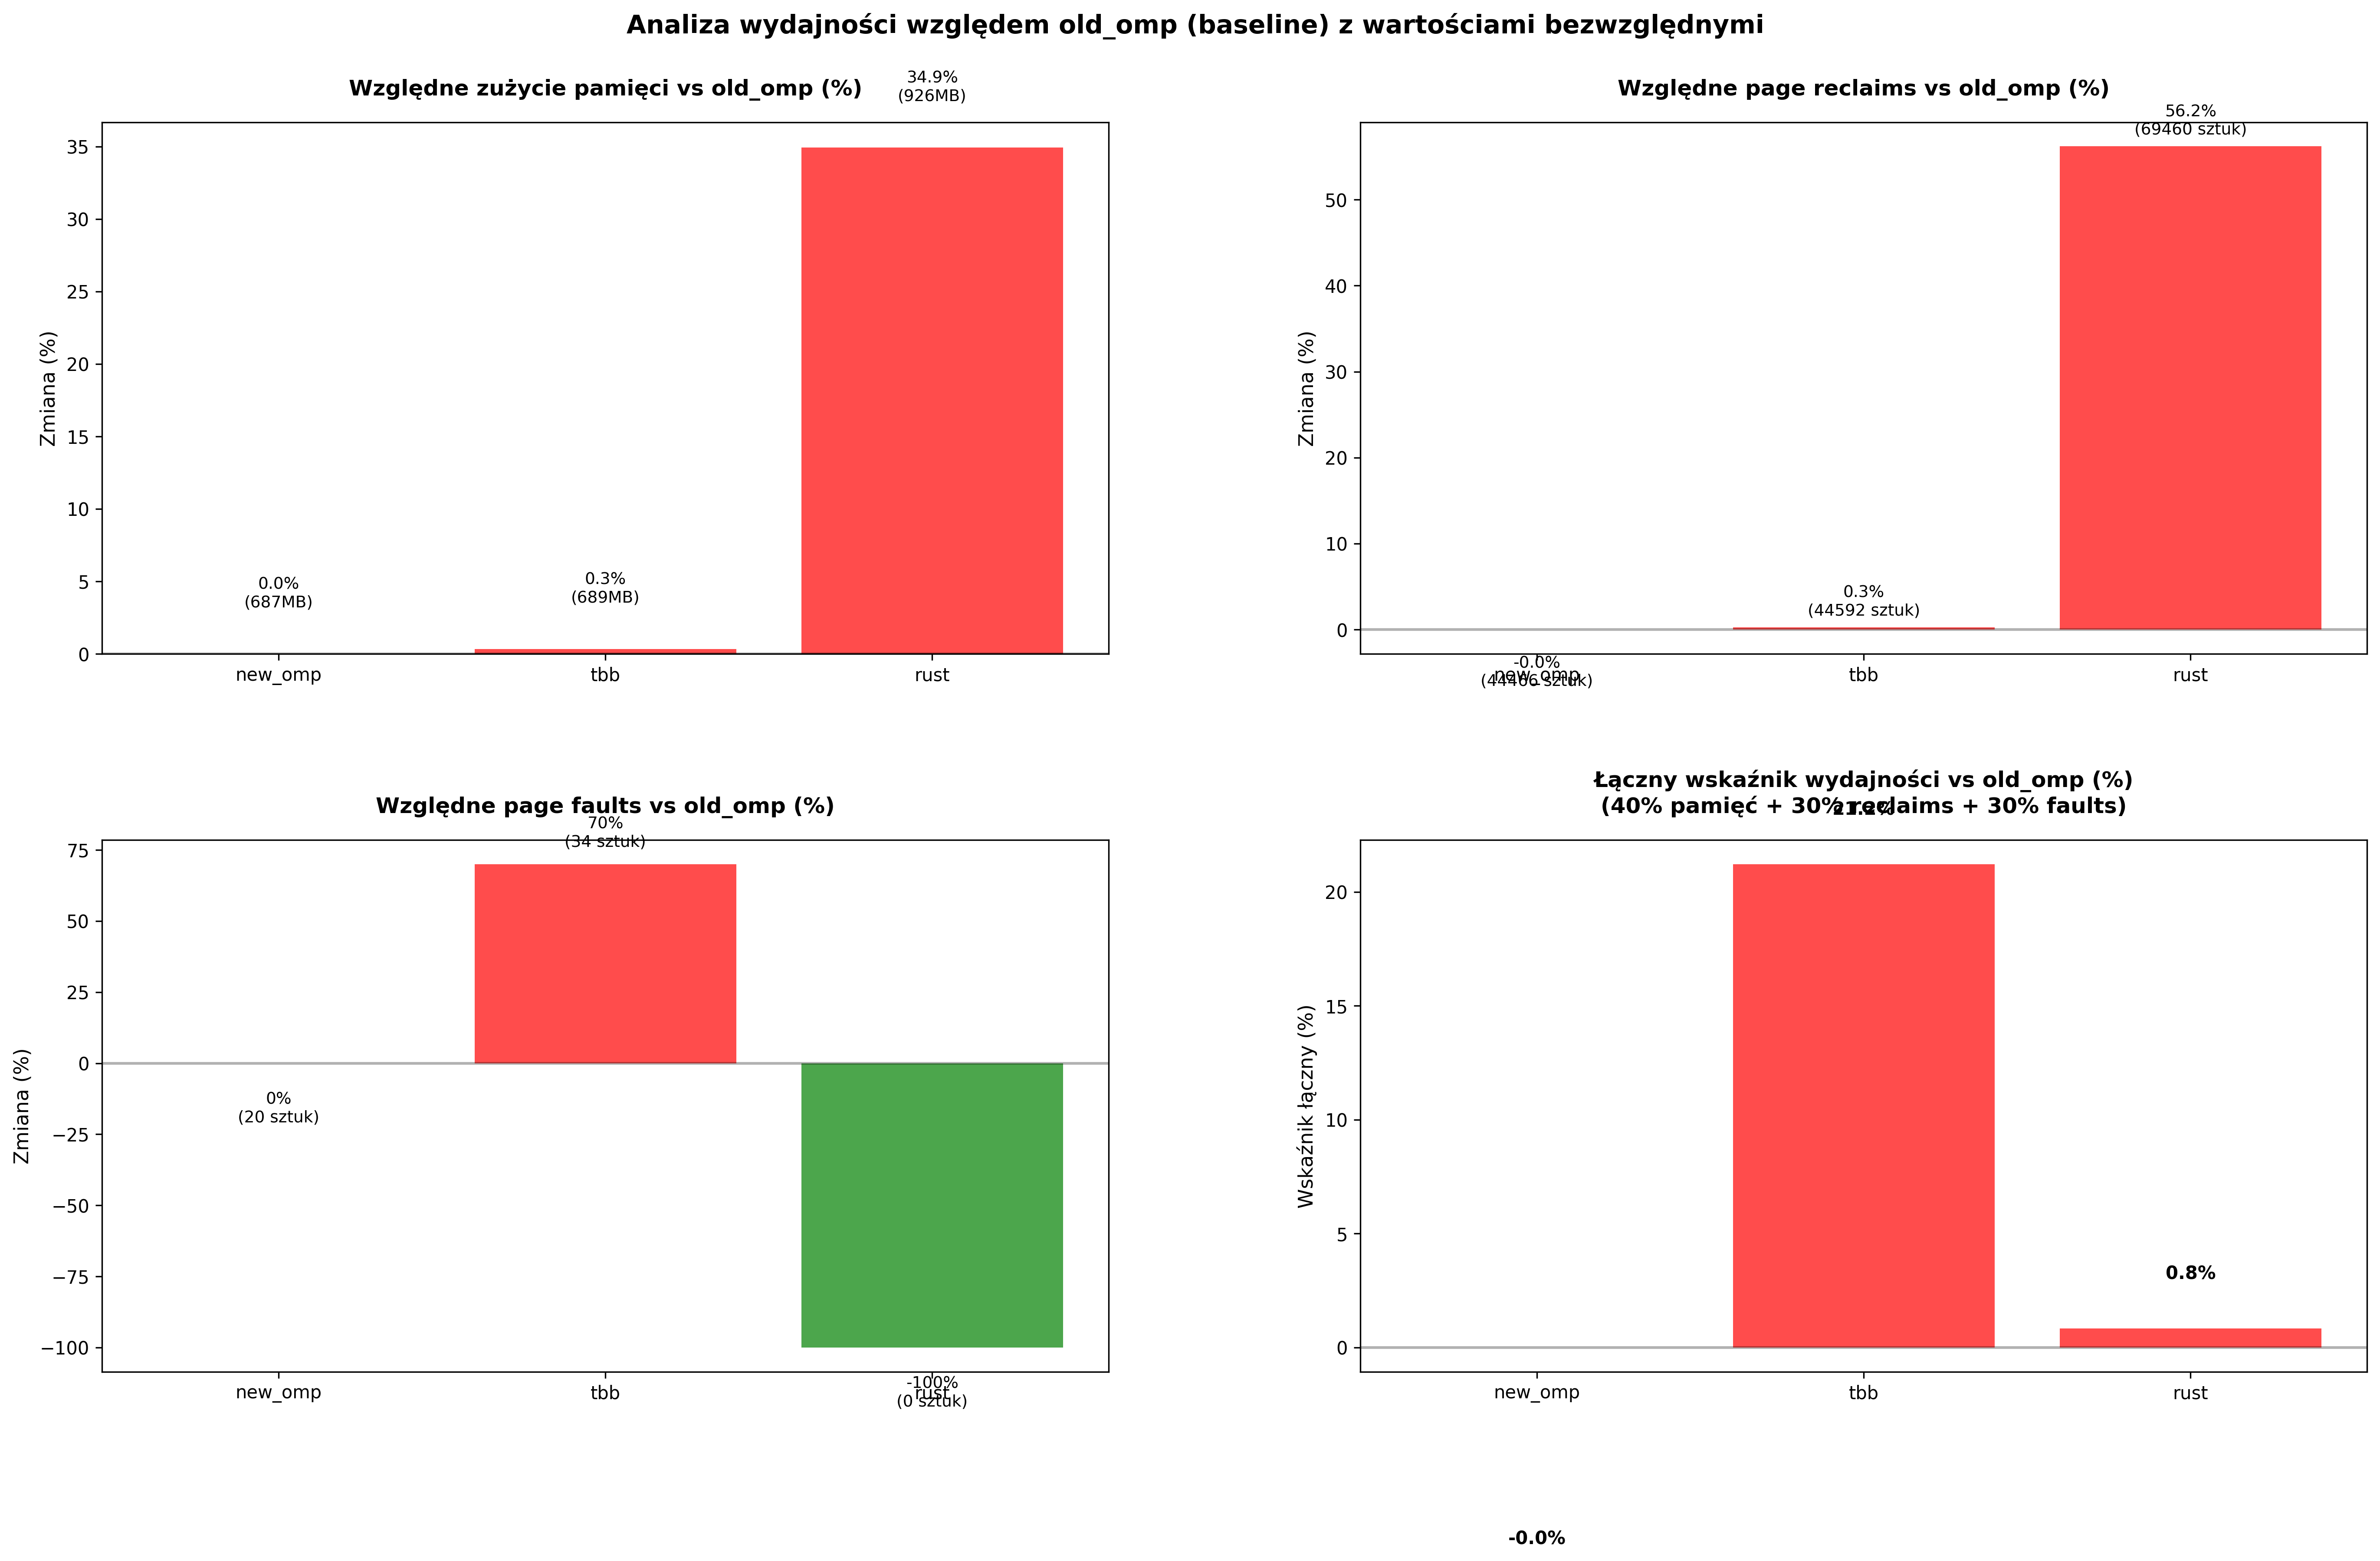
\includegraphics[width=\textwidth]{analiza/images/parallel/is/chart_05_performance_ratios.png}
    \caption{Analiza wydajności względem old\_omp (punkt odniesienia) z wartościami bezwzględnymi}
    \label{is_analiza_wzgledem_old_omp}
\end{figure}
Wykres ten - rysunek \ref{is_analiza_wzgledem_old_omp} przedstawia zmiany procentowe trzech kluczowych metryk względem wersji odniesienia (old\_omp):
\begin{itemize}
    \item Zużycie pamięci: new\_omp nie różni się w ogóle od wersji odniesienia (0\%), tbb wykazuje jedynie symboliczny wzrost (0,3\%), natomiast rust zużywa aż 34,9\% więcej pamięci.
    \item Odzyskiwanie stron pamięci: rust generuje aż 56,2\% więcej operacji odzyskania niż old\_omp, co stanowi znaczące obciążenie podsystemu pamięci.
    \item Błędy stron: rust jako jedyna implementacja całkowicie je eliminuje (-100\% względem old\_omp), co jest jej największym atutem oraz potwierdza założenia co do mechanizmów języka.
    \item Wskaźnik zbiorczy (ważony: 40\% pamięć + 30\% reclaims + 30\% faults) wskazuje, że jedynie tbb osiąga nieznaczną przewagę względem wersji bazowej (+0,8\%), natomiast rust wypada niekorzystnie pomimo doskonałej obsługi błędów, głównie przez nadmierne zużycie pamięci.
\end{itemize}



\begin{figure}[H]
    \centering
    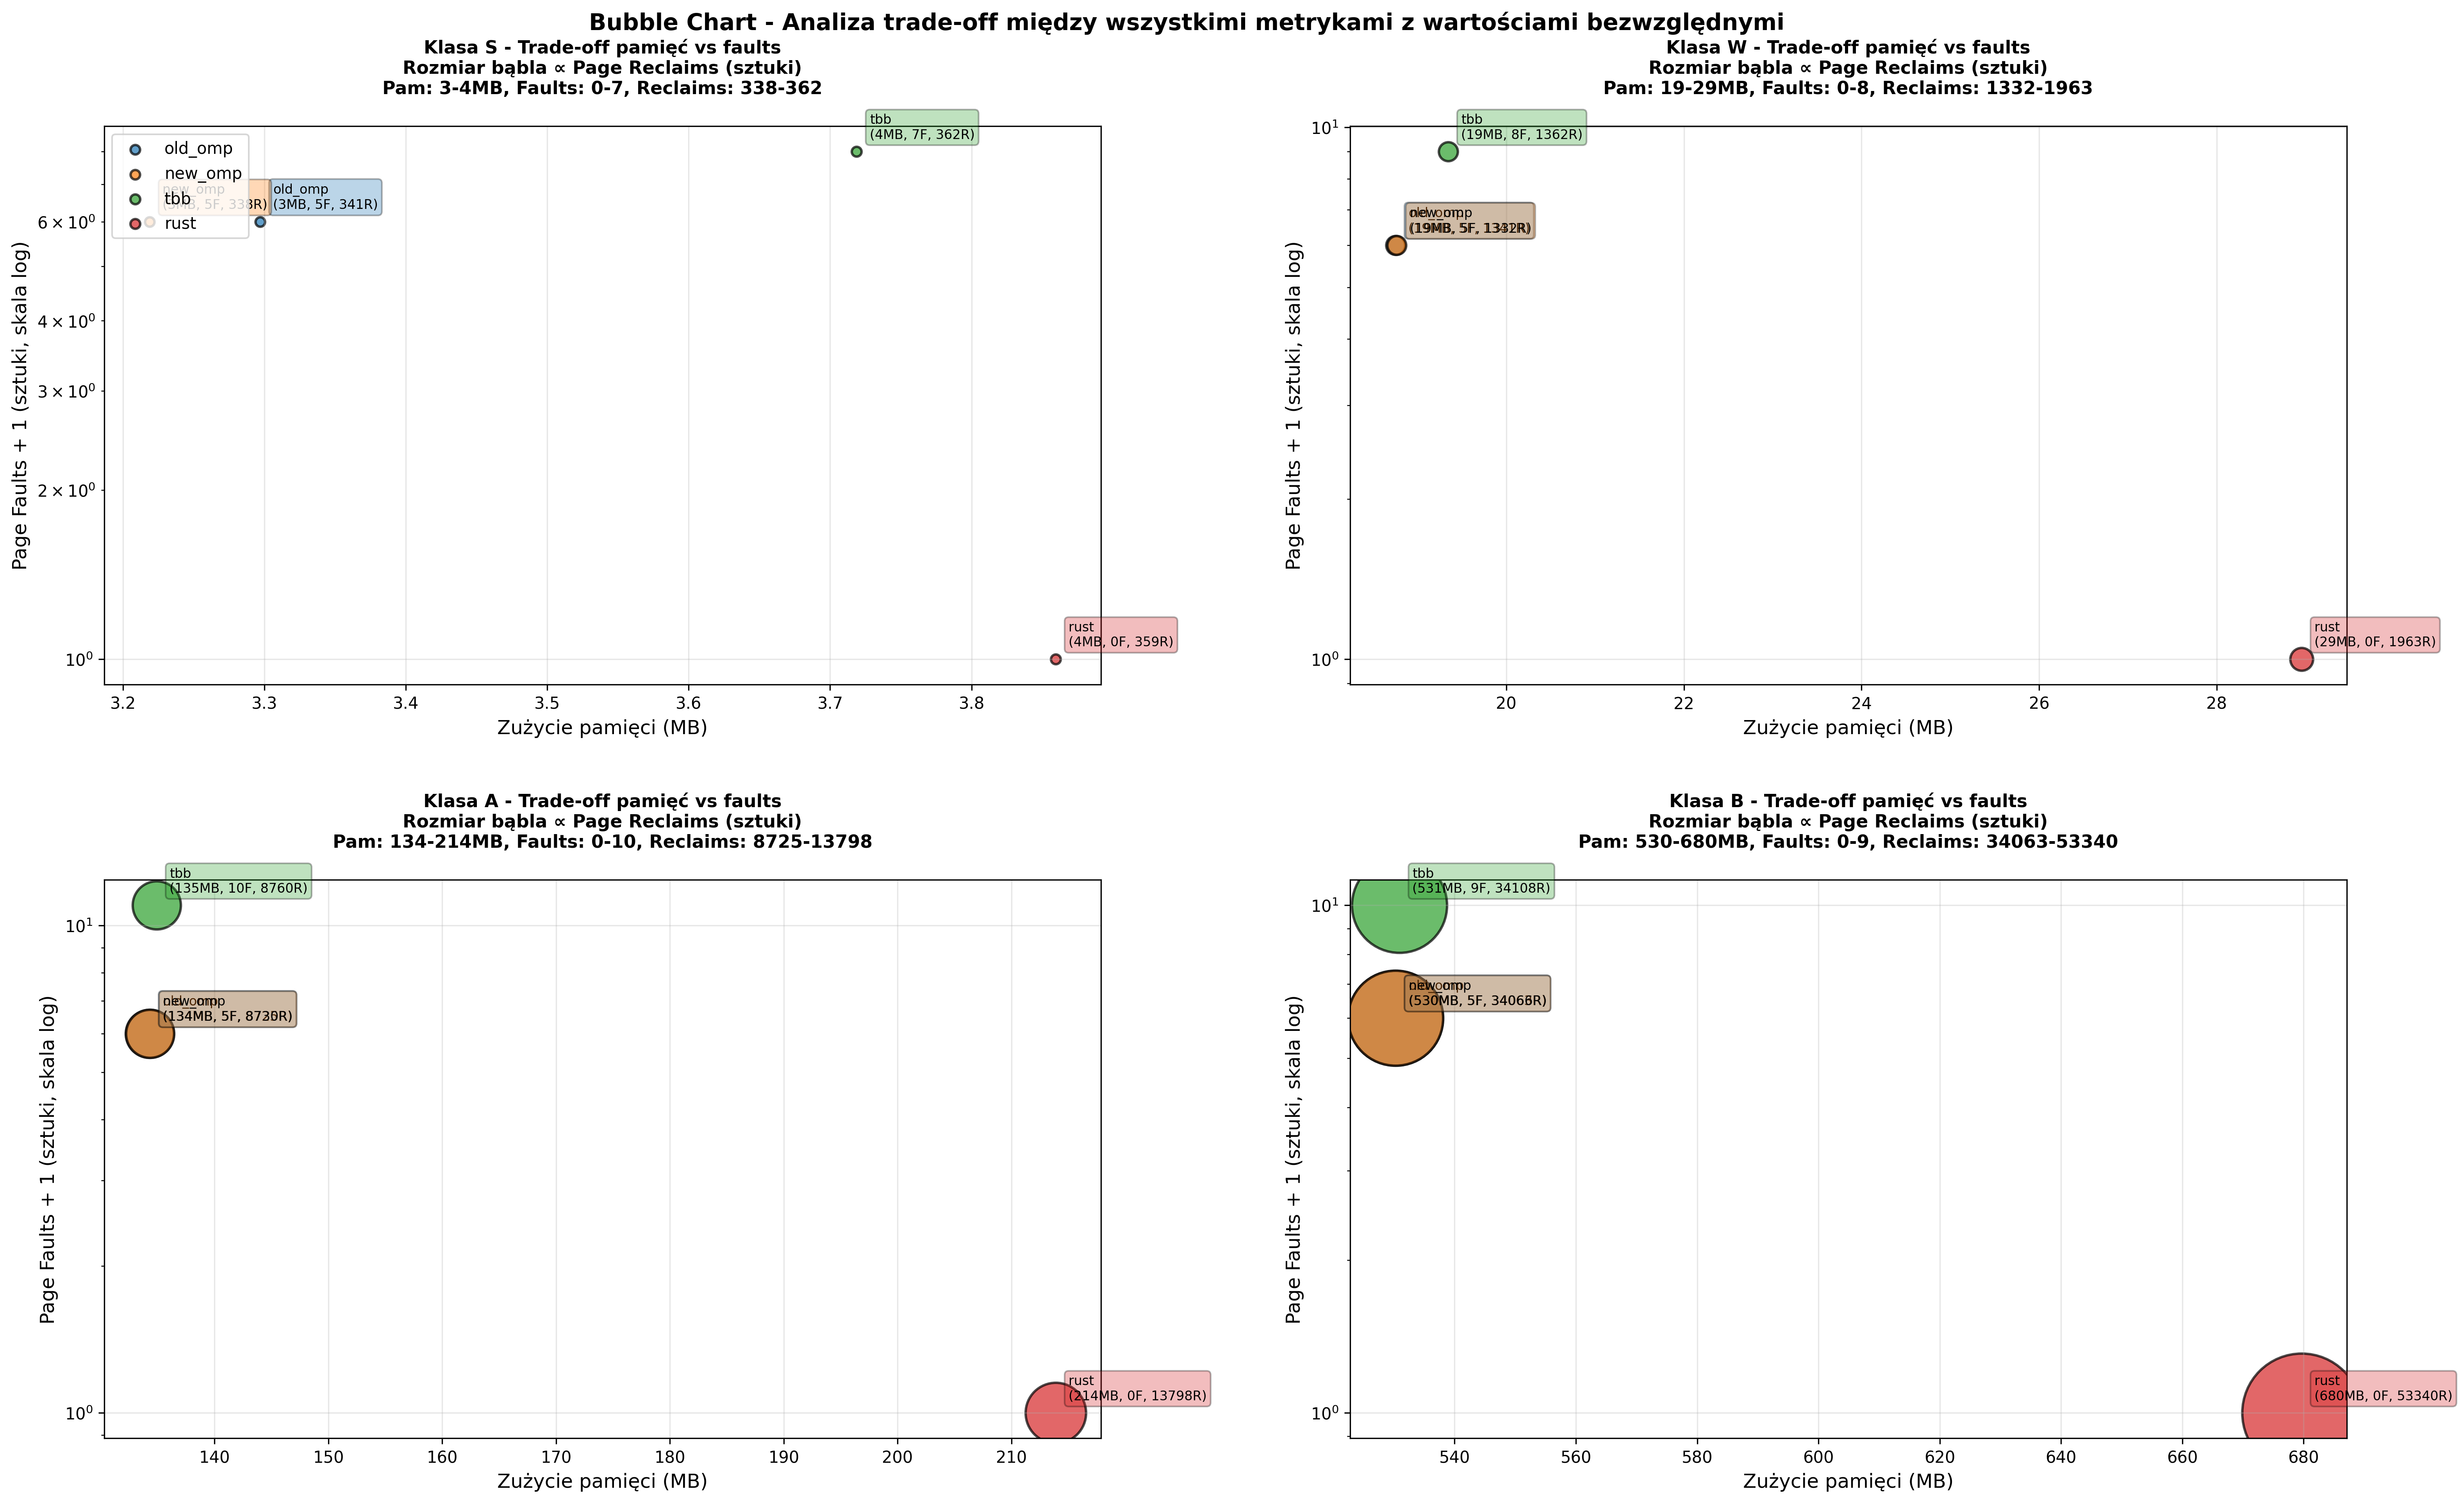
\includegraphics[width=\textwidth]{analiza/images/parallel/is/chart_06_bubble_chart.png}
    \caption{Kompromisy \eng{trade-off} pomiędzy zużyciem pamięci a błędami stron pamięci, z uwzględnieniem liczby odzyskanych stron jako trzeciej zmiennej reprezentowanej przez rozmiar bąbla}
    \label{is_kompromisy_pamiec_bledy}
\end{figure}
Na podstawie wykresu bąbelkowego - rysunek \ref{is_kompromisy_pamiec_bledy} można zauważyć:
\begin{itemize}
    \item rust w każdej klasie lokuje się w dolnym rejonie wykresu (niska liczba błędów) przy wysokim zużyciu pamięci oraz największych bąblach (najwięcej zwolnień stron).
    \item tbb regularnie generuje najwyższą liczbę błędów stron przy zbliżonym zużyciu pamięci jak old\_omp i new\_omp.
    \item new\_omp uzyskuje relatywnie zrównoważony kompromis – umiarkowane zużycie pamięci, średnia liczba błędów stron i średnia liczba odzyskanych stron.
\end{itemize}
\subsection{Wyniki profilowania wydajności - platforma x86\_64}